\documentclass{exam}
\usepackage{main}

\qformat{\emph{Question \thequestion}\hfill}

\title{Modèle de propagation d'une rumeur}
\date{4 Avril 2024}
\author{Maths Spécifiques}

\begin{document}
\maketitle
\section{Introduction}
Depuis la Seconde Guerre mondiale, la prolifération de rumeurs a engendré
des effets désastreux et les chercheurs se sont alors intéressés à leur
propagation. Aujourd'hui, avec les multiples sources d'information et
l'utilisation généralisée des réseaux sociaux, les vitesses de propagation de ces
rumeurs ont considérablement augmenté. La maîtrise du savoir étant un enjeu
essentiel pour les sociétés, il est important d'être capable de modéliser cette
propagation pour en comprendre le fonctionnement afin de distinguer une
information fondée d'une information fausse.

\section{Premier modèle}

On modélise la transmission d'une rumeur par le modèle suivant.

\begin{tcolorbox}
\begin{itemize}
\item Il y a trois types de personnes : Propagateur, Renseigné et Ignorant.
\item Initialement, il y a $p$ Propagateurs. Le reste de la population est Ignorante.
\item Chaque minute, tous les Propagateurs transmettent la rumeur à $q$ Ignorants.
\item Une fois la rumeur transmise, un Propagateur devient Renseigné.
\item Une fois la rumeur entendue, un Ignorant devient Propagateur.
\end{itemize}
\end{tcolorbox}
\vspace*{0.5cm}

\begin{questions}
\question On suppose pour commencer que $a = 1$ et $q = 2$. L'arbre suivant représente l'ensemble du phénomène au bout de $4$ minutes.
\begin{center}
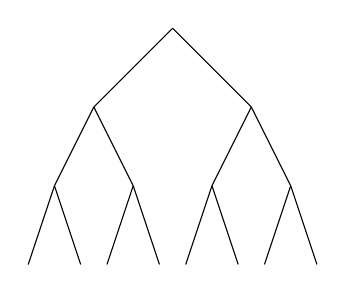
\begin{tikzpicture}
[level distance=1cm,level/.style={sibling distance=2cm/#1}]
\coordinate
child foreach \x in {0,1}
    {child foreach \y in {0,1}
        {child foreach \z in {0,1}}};
\end{tikzpicture}
\end{center}
Combien de personnes sont au courant de la rumeur au bout de $4$ minutes ? Quels noeuds de l'arbre correspondent aux Propagateurs et aux Renseignés ?
\makeemptybox{2cm}
\question Prolonger et compléter le tableau suivant.
\begin{center}
\begin{tabular}{|c|c|c|c|}
\hline
Minutes & Propagateurs & Renseignés & Total\\
\hline
0 & 1 & 0 & 1\\
\hline
1 & 2 & 1 & 3\\
\hline
2 & 4 & 3 & 7\\
\hline
&  &  & \\
\hline
\end{tabular}
\end{center}
\makeemptybox{2cm}
\question Combien de personnes ont eu connaissance de la rumeur au bout de $1$ minute ? $3$ minutes ? $5$ minutes ? $10$ minutes ?
\makeemptybox{2cm}
\question Soit $(u_n)$ la suite décrivant le nombre de propagateurs au bout de $n$ minutes. Donner une expression de $u_n$ en fonction de $n$. Quel est le nom de cette suite ?
\makeemptybox{2cm}
\question De par ce modèle, le nombre de personnes au courant de la rumeur au bout de $n$ minutes est donné par la formule
\begin{equation*}
p \times \dfrac{q^{n+1} - 1}{q - 1}
\end{equation*}
Pour les valeurs de $p$ et de $q$ suivantes, donner la transmission la plus rapide d'après ce modèle.
\begin{itemize}
\item $p=10$ et $q=2$;
\item $p=1$ et $q=3$. 
\end{itemize}
\makeemptybox{4cm}
\newpage
\section{Limites du premier modèle}
\question On suppose encore que $p = 1$ et $q = 2$. Combien de personnes sont au courant de la rumeur au bout de $10$ minutes et $30$ secondes ?
\makeemptybox{2cm}
Le modèle continu nous permet donc de considérer la quantité de personnes au courant de la rumeur à n'\emph{importe quel instant $t$}. On note donc $f(t)$ le nombre de personnes au courant à l'instant $t$.
\question Dans le cas où $p=1$ et $q=2$, la représentation graphique de $f$ est donnée par
\begin{center}
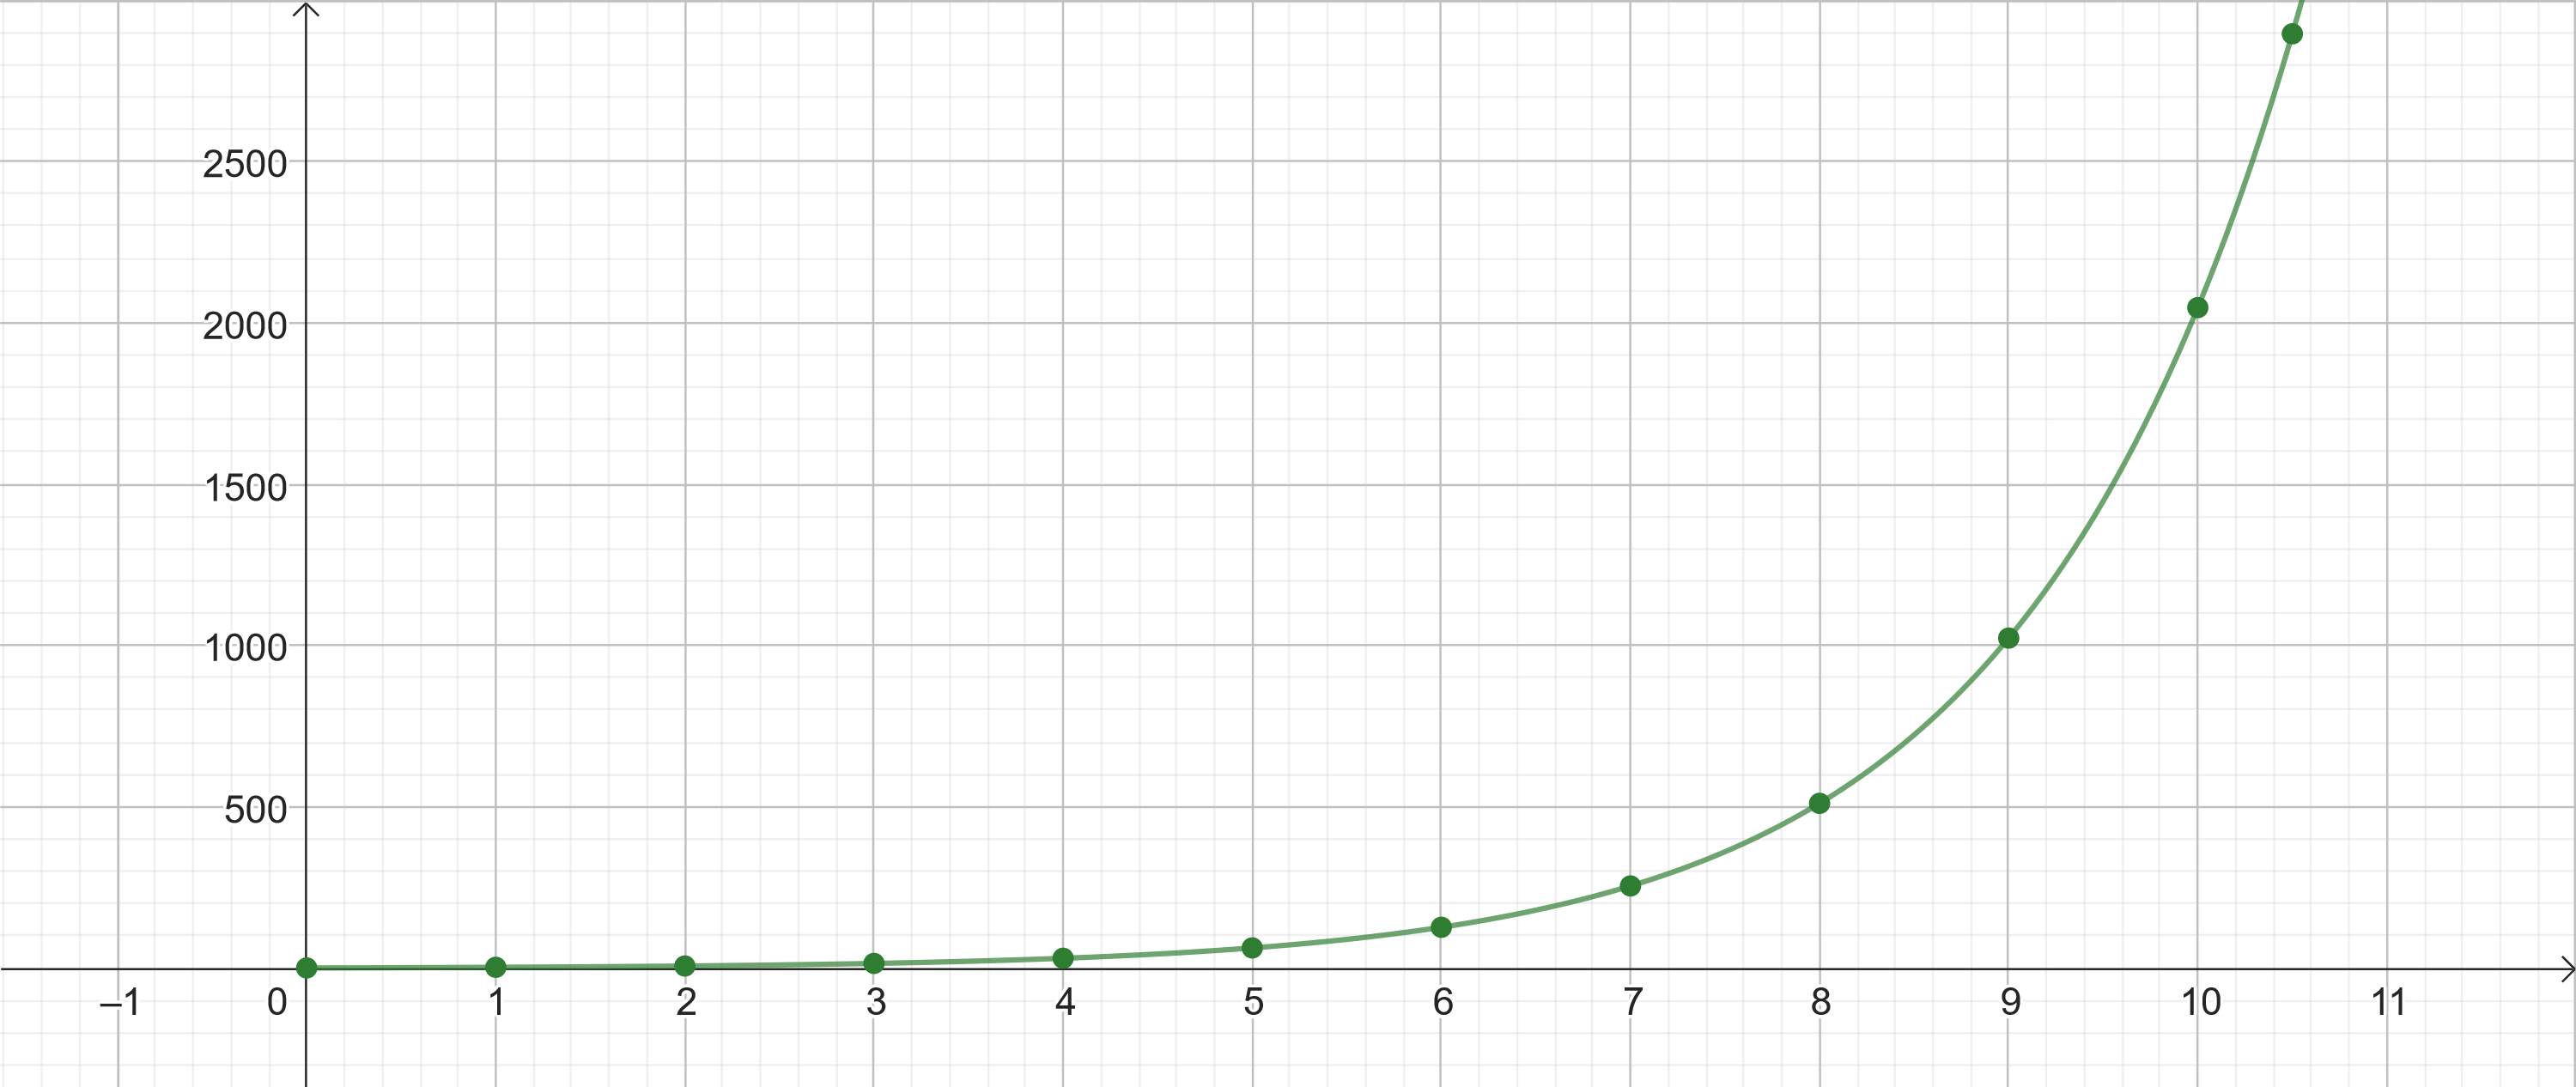
\includegraphics[scale=1]{Modele.png}
\end{center}
À partir de combien de temps $1500$ personnes sont au courant ? Cela vous paraît-il réaliste ?
\question Donner cinq raisons pour lesquelles ce modèle n'est pas réaliste selon vous.
\makeemptybox{4cm}
\end{questions}
\end{document}